
%(BEGIN_QUESTION)
% Copyright 2011, Tony R. Kuphaldt, released under the Creative Commons Attribution License (v 1.0)
% This means you may do almost anything with this work of mine, so long as you give me proper credit

Examine this process trend, showing the response of the process variable to a 10\% up-and-down step change in the controller output (placed in manual mode):

$$\includegraphics[width=15.5cm]{i01720x01.eps}$$

What characteristics of the process (and its related instrumentation) can you discern from this trend?  Based on this information, hypothesize how you think the controller should be tuned to respond.  In other words, how aggressive should the controller's P, I, and D terms be relative to each other?

\vfil 

\underbar{file i01720}
\eject
%(END_QUESTION)





%(BEGIN_ANSWER)

This is a graded question -- no answers or hints given!

%(END_ANSWER)





%(BEGIN_NOTES)

This is a trick question.  The process variable does not seem to be responding at all to the output.  Something is terribly wrong here, and it must be repaired before there is any hope of tuning the controller.

%INDEX% Control, PID tuning: predicting PID requirements based on open-loop response

%(END_NOTES)


